\section{Strategie per la progettazione concettuale}

Lo sviluppo di uno \textbf{schema concettuale} può essere considerato a tutti gli effetti un \textbf{processo di ingegnerizzazione}, in quanto richiede un insieme di fasi metodiche e ragionate per trasformare le specifiche di un problema reale in una rappresentazione astratta ma coerente e precisa.  

In altre parole, progettare uno schema concettuale non significa solo disegnare entità e relazioni, ma \textbf{analizzare, organizzare e strutturare le informazioni} in modo sistematico, seguendo principi simili a quelli utilizzati nell’ingegneria del software.

\begin{tcolorbox}[colback=yellow!20,colframe=yellow!50!black,title={\textbf{Nota Bene}},boxrule=0.8pt,arc=2mm]
Per \textbf{ingegnerizzazione} si intende l’\textit{applicazione di un metodo rigoroso e pianificato} alla progettazione, allo sviluppo e alla verifica di un sistema complesso.  
Nel contesto della modellazione dei dati, ciò significa:  
\begin{itemize}
  \item partire da requisiti chiari e ben definiti;
  \item progettare in modo graduale e controllato (Top-Down, Bottom-Up o Inside-Out);
  \item assicurarsi che lo schema finale sia corretto, completo e privo di ambiguità.
\end{itemize}
\end{tcolorbox}

\begin{center}
\textit{Ricorda che uno schema concettuale è una rappresentazione astratta e indipendente dal linguaggio di implementazione, che descrive le informazioni e le relazioni fondamentali di un sistema informativo.}
\end{center}

% -------------------------------------------------
\subsection{Strategia Top-Down}

La strategia \textbf{Top-Down} consiste nel partire da una \textbf{visione globale del sistema} e procedere verso una \textbf{maggiore specificazione dei dettagli}.  
È un approccio deduttivo: si comincia con concetti generali e astratti per poi raffinarli gradualmente fino a ottenere uno schema concettuale completo e preciso.

\begin{itemize}
  \item \textbf{Fase 1:} considerare le specifiche globalmente e produrre uno schema iniziale \textbf{completo ma con pochi concetti astratti}.  
  \item \textbf{Fase 2:} \textbf{raffinare} progressivamente i concetti astratti fino ad arrivare a uno schema concettuale \textbf{dettagliato in ogni parte}.
\end{itemize}

\begin{tcolorbox}[colback=yellow!20,colframe=yellow!50!black,title={\textbf{Nota Bene}},boxrule=0.8pt,arc=2mm]
La strategia Top-Down è particolarmente utile quando si ha una visione chiara e globale del dominio applicativo.  
Permette di mantenere coerenza tra le parti del progetto, ma richiede una buona capacità di astrazione e pianificazione.
\end{tcolorbox}

\begin{center}
\textit{Esempio:} prima si individuano le entità principali (\textit{Studente}, \textit{Corso}, \textit{Docente}), poi si aggiungono relazioni e attributi specifici come \textit{data di nascita}, \textit{esame sostenuto}, \textit{voto}, ecc.
\end{center}

% -------------------------------------------------
\subsection{Strategia Bottom-Up}

La strategia \textbf{Bottom-Up} adotta un approccio opposto rispetto al Top-Down.  
In questo caso si parte dai \textbf{dettagli elementari} per poi integrarli progressivamente fino a ottenere la visione complessiva del sistema.  
È un metodo \textbf{induttivo}, ideale quando si dispone di molte informazioni di base ma non ancora di una struttura generale.

\begin{itemize}
  \item \textbf{Fase 1:} \textbf{decomporre} le specifiche iniziali in \textbf{parti elementari}, ovvero piccole frasi o porzioni di testo che descrivono uno stesso concetto o una singola informazione.  
  \item \textbf{Fase 2:} \textbf{generare gli schemi} per ciascuna parte elementare individuata.  
  \item \textbf{Fase 3:} \textbf{fondere gli schemi} parziali introducendo, se necessario, altri costrutti del modello E-R, in modo da \textbf{integrare} tutti gli elementi e ottenere lo \textbf{schema finale}.
\end{itemize}

\begin{tcolorbox}[colback=yellow!20,colframe=yellow!50!black,title={\textbf{Nota Bene}},boxrule=0.8pt,arc=2mm]
La strategia Bottom-Up è utile quando le specifiche non sono complete o sono distribuite in frammenti separati.  
Permette di costruire lo schema passo dopo passo, ma richiede attenzione nella fase di integrazione per evitare ridondanze o incoerenze tra i diversi schemi parziali.
\end{tcolorbox}

\begin{center}
\textit{Esempio:} si analizzano prima frasi come “uno studente sostiene un esame” o “un docente insegna un corso”, si crea uno schema per ciascuna, e infine si uniscono tutti in un unico schema concettuale completo.
\end{center}

% -------------------------------------------------
\subsection{Strategia Inside-Out}

La strategia \textbf{Inside-Out} rappresenta un approccio intermedio rispetto a Top-Down e Bottom-Up.  
Si parte da alcuni \textbf{concetti centrali o fondamentali} del dominio, detti \textbf{concetti guida}, e si costruisce lo schema espandendolo progressivamente verso l’esterno.

\begin{itemize}
  \item \textbf{Fase 1:} \textbf{individuare} nelle specifiche alcuni concetti importanti, detti \textbf{concetti guida}.  
  \item \textbf{Fase 2:} \textbf{generare gli schemi} relativi ai concetti guida scelti.  
  \item \textbf{Fase 3:} \textbf{fondere gli schemi} precedenti e aggiungere gradualmente gli altri concetti fino a ottenere lo \textbf{schema concettuale completo}.
\end{itemize}

\begin{tcolorbox}[colback=yellow!20,colframe=yellow!50!black,title={\textbf{Nota Bene}},boxrule=0.8pt,arc=2mm]
La strategia Inside-Out è utile quando si riescono a identificare con chiarezza alcuni elementi chiave del sistema.  
Permette di concentrarsi inizialmente sulle parti più rilevanti e poi di estendere lo schema, garantendo coerenza e controllo durante l’espansione.
\end{tcolorbox}

\begin{center}
\textit{Esempio:} si parte dai concetti guida come \textit{Studente} e \textit{Corso}, si definiscono le loro relazioni principali, e poi si estende lo schema aggiungendo altri concetti come \textit{Esame}, \textit{Docente} o \textit{Dipartimento}.
\end{center}

% -------------------------------------------------
\subsection{Analisi di qualità dello schema}

L’\textbf{analisi di qualità} di uno schema concettuale serve a valutare se il modello prodotto rappresenta correttamente e in modo efficace il dominio di interesse.  
Essa comprende quattro aspetti fondamentali:
\begin{itemize}
  \item Verifica di correttezza
  \item Verifica di completezza
  \item Verifica di minimalità
  \item Verifica di leggibilità
\end{itemize}

\textbf{Verifica di correttezza}  
Uno schema concettuale è \textbf{corretto} se utilizza propriamente i costrutti del modello concettuale adottato (nel nostro caso, il modello E-R).  
La correttezza si valuta controllando che lo schema rispetti le regole sintattiche e semantiche del modello.

\begin{itemize}
  \item \textbf{Errori sintattici:} utilizzo scorretto dei costrutti del modello E-R, senza rispettarne le regole formali.  
  \textit{Esempi:}
  \begin{itemize}
    \item introduzione di una generalizzazione di relazioni;
    \item relazioni non collegate ad alcuna entità;
    \item relazioni che possiedono un identificatore.
  \end{itemize}
  
  \item \textbf{Errori semantici (errori d’uso):} uso improprio dei costrutti del modello, senza rispettarne il significato.  
  \textit{Esempi:}
  \begin{itemize}
    \item uso di una relazione per rappresentare un concetto che dovrebbe essere un’entità autonoma;
    \item uso di un attributo per rappresentare un concetto complesso o collegato ad altri concetti in più punti dello schema.
  \end{itemize}
\end{itemize}

\textbf{Verifica di completezza e minimalità}  
Uno schema concettuale è \textbf{completo} se rappresenta tutte le informazioni di interesse e consente di eseguire tutte le operazioni previste dalle specifiche.  
È invece \textbf{minimale} quando tutti i concetti presenti nei requisiti sono rappresentati una sola volta, evitando ridondanze o duplicazioni.

\textbf{Verifica di leggibilità}  
La leggibilità riguarda la \textbf{chiarezza e l’organizzazione visiva} dello schema.  
Uno schema ben leggibile deve essere ordinato, coerente e facilmente interpretabile anche da chi non lo ha progettato.

\begin{tcolorbox}[colback=yellow!20,colframe=yellow!50!black,title={\textbf{Nota Bene}},boxrule=0.8pt,arc=2mm]
Un buon schema concettuale deve essere:
\begin{itemize}
  \item \textbf{Corretto} → rispetta le regole sintattiche e semantiche del modello E-R;
  \item \textbf{Completo} → include tutte le informazioni richieste;
  \item \textbf{Minimale} → evita ridondanze e duplicazioni;
  \item \textbf{Leggibile} → chiaro, ordinato e facilmente comprensibile.
\end{itemize}
Solo quando tutte queste condizioni sono soddisfatte, lo schema può essere considerato di \textbf{alta qualità}.
\end{tcolorbox}

% -------------------------------------------------
\subsection{Ridondanze}

Uno \textbf{schema concettuale non minimale} può contenere delle \textbf{ridondanze}, ossia rappresentazioni multiple dello stesso concetto logico.  
I casi più comuni di ridondanza sono:

\begin{itemize}
    \item \textbf{Ereditarietà delle relazioni}
    \item \textbf{Cicli di relazioni}
\end{itemize}

\begin{figure}[!h]
    \centering
    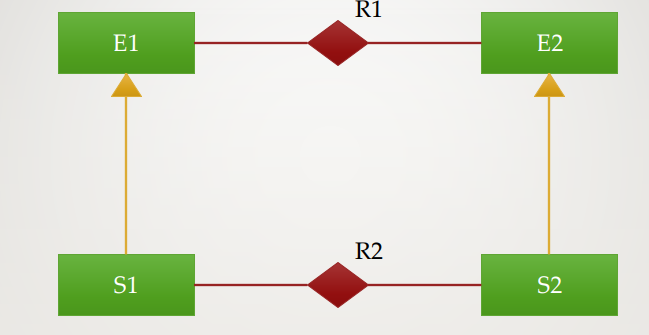
\includegraphics[width=0.55\linewidth]{image19.png}
    \caption{Ereditarietà delle relazioni}
    \label{fig:ereditarieta-relazioni}
\end{figure}

\begin{center}
È \textbf{probabile, ma non certo}, che la relazione \textit{R2} sia ridondante.  
Va quindi verificato se \textit{R2} rappresenti lo stesso legame logico già espresso da \textit{R1}; se così fosse, \textit{R2} deve essere eliminata in quanto effettivamente ridondante.
\end{center}

\begin{figure}[!h]
    \centering
    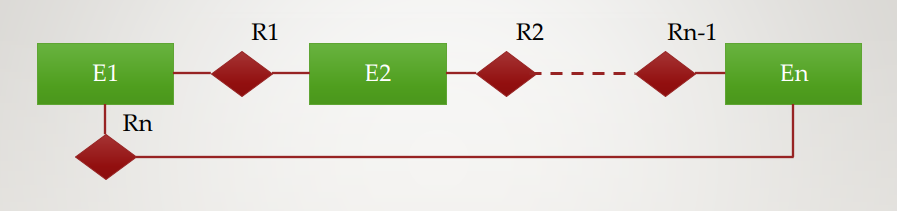
\includegraphics[width=0.75\linewidth]{image20.png}
    \caption{Ciclo di relazioni}
    \label{fig:ciclo-relazioni}
\end{figure}

\begin{center}
È \textbf{probabile, ma non certo}, che una delle relazioni $R_i$ sia ridondante.  
Va quindi verificato se la relazione $R_i$ possa essere ottenuta \textbf{dalla composizione delle altre relazioni}.  
Se così fosse, $R_i$ deve essere eliminata in quanto effettivamente ridondante.
\end{center}

% -------------------------------------------------
\subsection{Semplificazioni dello schema}

Non sempre le \textbf{relazioni ternarie} sono facili da leggere e interpretare; per questo motivo, la loro eliminazione può talvolta migliorare la \textbf{leggibilità dello schema concettuale}.  

Le seguenti operazioni possono essere applicate per semplificare o trasformare una relazione ternaria:

\begin{itemize}
  \item \textbf{Trasformazione di una relazione ternaria in un’entità}  
  Questa operazione è \textbf{sempre applicabile} e consiste nel sostituire la relazione ternaria con una nuova entità, collegata tramite relazioni binarie alle entità originarie.  

  \item \textbf{Riduzione di una relazione ternaria a due relazioni binarie}  
  Questa operazione è possibile solo se una delle entità coinvolte partecipa alla relazione ternaria con \textbf{cardinalità (1,1)}.  
  In tal caso, la relazione ternaria può essere sostituita da due relazioni binarie equivalenti, mantenendo il significato logico dello schema.
\end{itemize}

\begin{tcolorbox}[colback=yellow!20,colframe=yellow!50!black,title={\textbf{Nota Bene}},boxrule=0.8pt,arc=2mm]
La trasformazione o riduzione delle relazioni ternarie deve essere eseguita con attenzione:  
l’obiettivo è migliorare la leggibilità dello schema senza alterarne il significato semantico.
\end{tcolorbox}

\begin{figure}[!h]
    \centering
    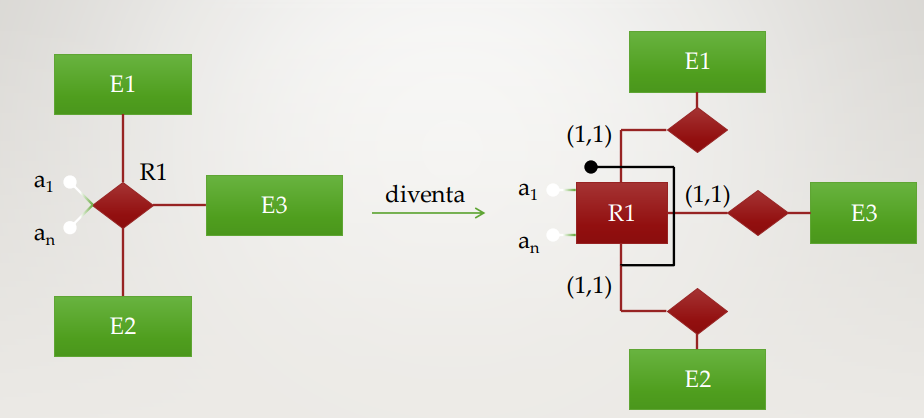
\includegraphics[width=0.75\linewidth]{image21.png}
    \caption{Trasformazione di una relazione ternaria in un’entità}
    \label{fig:relazione-ternaria-entita}
\end{figure}

\begin{figure}[H]
    \centering
    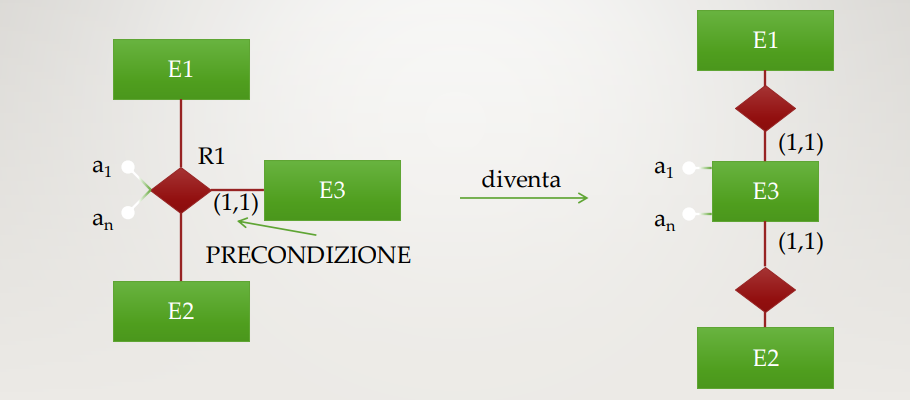
\includegraphics[width=0.75\linewidth]{image22.png}
    \caption{Riduzione di una relazione ternaria a due relazioni binarie}
    \label{fig:relazione-ternaria-binarie}
\end{figure}
Un ulteriore miglioramento nella leggibilità si ottiene esplicitando, nelle \textbf{generalizzazioni sovrapposte}, l’entità che rappresenta la sovrapposizione.  
In questo modo, la generalizzazione sovrapposta viene trasformata in una \textbf{generalizzazione esclusiva}, rendendo lo schema più chiaro e facilmente interpretabile.

